% Created by tikzDevice version 0.6.1 on 2011-06-26 17:52:49
% !TEX encoding = UTF-8 Unicode
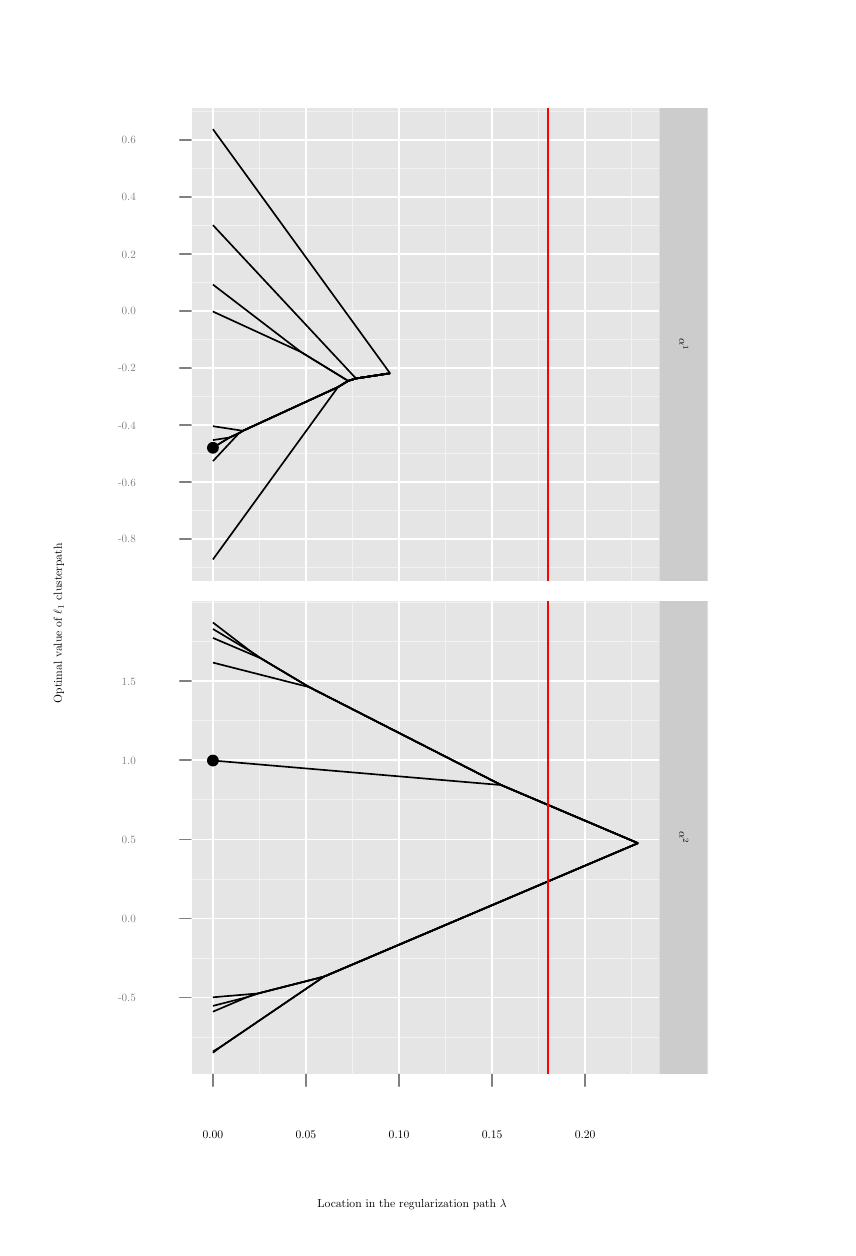
\begin{tikzpicture}[x=1pt,y=1pt]
\definecolor[named]{drawColor}{rgb}{0.00,0.00,0.00}
\definecolor[named]{fillColor}{rgb}{1.00,1.00,1.00}
\fill[color=fillColor,] (0,0) rectangle (289.08,433.62);
\begin{scope}
\path[clip] (  0.00,  0.00) rectangle (289.08,433.62);
\end{scope}
\begin{scope}
\path[clip] (  0.00,  0.00) rectangle (289.08,433.62);
\end{scope}
\begin{scope}
\path[clip] (  0.00,  0.00) rectangle (289.08,433.62);
\end{scope}
\begin{scope}
\path[clip] (  0.00,  0.00) rectangle (289.08,433.62);
\end{scope}
\begin{scope}
\path[clip] (  0.00,  0.00) rectangle (289.08,433.62);
\end{scope}
\begin{scope}
\path[clip] (  0.00,  0.00) rectangle (289.08,433.62);
\end{scope}
\begin{scope}
\path[clip] (  0.00,  0.00) rectangle (289.08,433.62);
\end{scope}
\begin{scope}
\path[clip] (  0.00,  0.00) rectangle (289.08,433.62);
\end{scope}
\begin{scope}
\path[clip] (  0.00,  0.00) rectangle (289.08,433.62);
\end{scope}
\begin{scope}
\path[clip] (  0.00,  0.00) rectangle (289.08,433.62);
\definecolor[named]{fillColor}{rgb}{1.00,1.00,1.00}

\draw[fill=fillColor,draw opacity=0.00,] (  0.00,  0.00) rectangle (289.08,433.62);
\end{scope}
\begin{scope}
\path[clip] (  0.00,  0.00) rectangle (289.08,433.62);
\end{scope}
\begin{scope}
\path[clip] (  0.00,  0.00) rectangle (289.08,433.62);
\definecolor[named]{drawColor}{rgb}{0.00,0.00,0.00}

\node[color=drawColor,anchor=base,inner sep=0pt, outer sep=0pt, scale=  0.42] at (138.90,  7.23) {Location in the regularization path $\lambda$%
};
\end{scope}
\begin{scope}
\path[clip] (  0.00,  0.00) rectangle (289.08,433.62);
\definecolor[named]{drawColor}{rgb}{0.00,0.00,0.00}

\node[rotate= 90.00,color=drawColor,anchor=base,inner sep=0pt, outer sep=0pt, scale=  0.42] at ( 12.37,218.39) {Optimal value of $\ell_1$ clusterpath%
};
\end{scope}
\begin{scope}
\path[clip] (  0.00,  0.00) rectangle (289.08,433.62);
\end{scope}
\begin{scope}
\path[clip] ( 32.08,404.71) rectangle ( 59.25,404.71);
\end{scope}
\begin{scope}
\path[clip] (  0.00,  0.00) rectangle (289.08,433.62);
\end{scope}
\begin{scope}
\path[clip] ( 32.08,404.71) rectangle ( 59.25,404.71);
\end{scope}
\begin{scope}
\path[clip] (  0.00,  0.00) rectangle (289.08,433.62);
\end{scope}
\begin{scope}
\path[clip] (  0.00,  0.00) rectangle (289.08,433.62);
\end{scope}
\begin{scope}
\path[clip] (  0.00,  0.00) rectangle (289.08,433.62);
\end{scope}
\begin{scope}
\path[clip] ( 32.08,226.45) rectangle ( 59.25,233.68);
\end{scope}
\begin{scope}
\path[clip] (  0.00,  0.00) rectangle (289.08,433.62);
\end{scope}
\begin{scope}
\path[clip] (  0.00,  0.00) rectangle (289.08,433.62);
\end{scope}
\begin{scope}
\path[clip] (  0.00,  0.00) rectangle (289.08,433.62);
\end{scope}
\begin{scope}
\path[clip] ( 32.08, 55.41) rectangle ( 59.25, 55.41);
\end{scope}
\begin{scope}
\path[clip] (  0.00,  0.00) rectangle (289.08,433.62);
\end{scope}
\begin{scope}
\path[clip] ( 32.08, 32.08) rectangle ( 59.25, 55.41);
\end{scope}
\begin{scope}
\path[clip] (  0.00,  0.00) rectangle (289.08,433.62);
\end{scope}
\begin{scope}
\path[clip] ( 32.08, 32.08) rectangle ( 59.25, 32.08);
\end{scope}
\begin{scope}
\path[clip] (  0.00,  0.00) rectangle (289.08,433.62);
\end{scope}
\begin{scope}
\path[clip] ( 59.25,404.71) rectangle ( 59.25,404.71);
\end{scope}
\begin{scope}
\path[clip] (  0.00,  0.00) rectangle (289.08,433.62);
\end{scope}
\begin{scope}
\path[clip] ( 59.25,404.71) rectangle ( 59.25,404.71);
\end{scope}
\begin{scope}
\path[clip] (  0.00,  0.00) rectangle (289.08,433.62);
\end{scope}
\begin{scope}
\path[clip] ( 59.25,233.68) rectangle ( 59.25,404.71);
\end{scope}
\begin{scope}
\path[clip] (  0.00,  0.00) rectangle (289.08,433.62);
\end{scope}
\begin{scope}
\path[clip] ( 59.25,226.45) rectangle ( 59.25,233.68);
\end{scope}
\begin{scope}
\path[clip] (  0.00,  0.00) rectangle (289.08,433.62);
\end{scope}
\begin{scope}
\path[clip] ( 59.25, 55.41) rectangle ( 59.25,226.45);
\end{scope}
\begin{scope}
\path[clip] (  0.00,  0.00) rectangle (289.08,433.62);
\end{scope}
\begin{scope}
\path[clip] ( 59.25, 55.41) rectangle ( 59.25, 55.41);
\end{scope}
\begin{scope}
\path[clip] (  0.00,  0.00) rectangle (289.08,433.62);
\end{scope}
\begin{scope}
\path[clip] ( 59.25, 32.08) rectangle ( 59.25, 55.41);
\end{scope}
\begin{scope}
\path[clip] (  0.00,  0.00) rectangle (289.08,433.62);
\end{scope}
\begin{scope}
\path[clip] ( 59.25, 32.08) rectangle ( 59.25, 32.08);
\end{scope}
\begin{scope}
\path[clip] (  0.00,  0.00) rectangle (289.08,433.62);
\end{scope}
\begin{scope}
\path[clip] ( 59.25,404.71) rectangle (228.22,404.71);
\end{scope}
\begin{scope}
\path[clip] (  0.00,  0.00) rectangle (289.08,433.62);
\end{scope}
\begin{scope}
\path[clip] ( 59.25,404.71) rectangle (228.22,404.71);
\end{scope}
\begin{scope}
\path[clip] (  0.00,  0.00) rectangle (289.08,433.62);
\end{scope}
\begin{scope}
\path[clip] ( 59.25,233.68) rectangle (228.22,404.71);
\end{scope}
\begin{scope}
\path[clip] (  0.00,  0.00) rectangle (289.08,433.62);
\end{scope}
\begin{scope}
\path[clip] ( 59.25,226.45) rectangle (228.22,233.68);
\end{scope}
\begin{scope}
\path[clip] (  0.00,  0.00) rectangle (289.08,433.62);
\end{scope}
\begin{scope}
\path[clip] ( 59.25, 55.41) rectangle (228.22,226.45);
\end{scope}
\begin{scope}
\path[clip] (  0.00,  0.00) rectangle (289.08,433.62);
\end{scope}
\begin{scope}
\path[clip] ( 59.25, 55.41) rectangle (228.22, 55.41);
\end{scope}
\begin{scope}
\path[clip] (  0.00,  0.00) rectangle (289.08,433.62);
\end{scope}
\begin{scope}
\path[clip] (  0.00,  0.00) rectangle (289.08,433.62);
\end{scope}
\begin{scope}
\path[clip] (  0.00,  0.00) rectangle (289.08,433.62);
\end{scope}
\begin{scope}
\path[clip] ( 59.25, 32.08) rectangle (228.22, 32.08);
\end{scope}
\begin{scope}
\path[clip] (  0.00,  0.00) rectangle (289.08,433.62);
\end{scope}
\begin{scope}
\path[clip] (228.22,404.71) rectangle (228.22,404.71);
\end{scope}
\begin{scope}
\path[clip] (  0.00,  0.00) rectangle (289.08,433.62);
\end{scope}
\begin{scope}
\path[clip] (228.22,404.71) rectangle (228.22,404.71);
\end{scope}
\begin{scope}
\path[clip] (  0.00,  0.00) rectangle (289.08,433.62);
\end{scope}
\begin{scope}
\path[clip] (228.22,233.68) rectangle (228.22,404.71);
\end{scope}
\begin{scope}
\path[clip] (  0.00,  0.00) rectangle (289.08,433.62);
\end{scope}
\begin{scope}
\path[clip] (228.22,226.45) rectangle (228.22,233.68);
\end{scope}
\begin{scope}
\path[clip] (  0.00,  0.00) rectangle (289.08,433.62);
\end{scope}
\begin{scope}
\path[clip] (228.22, 55.41) rectangle (228.22,226.45);
\end{scope}
\begin{scope}
\path[clip] (  0.00,  0.00) rectangle (289.08,433.62);
\end{scope}
\begin{scope}
\path[clip] (228.22, 55.41) rectangle (228.22, 55.41);
\end{scope}
\begin{scope}
\path[clip] (  0.00,  0.00) rectangle (289.08,433.62);
\end{scope}
\begin{scope}
\path[clip] (228.22, 32.08) rectangle (228.22, 55.41);
\end{scope}
\begin{scope}
\path[clip] (  0.00,  0.00) rectangle (289.08,433.62);
\end{scope}
\begin{scope}
\path[clip] (228.22, 32.08) rectangle (228.22, 32.08);
\end{scope}
\begin{scope}
\path[clip] (  0.00,  0.00) rectangle (289.08,433.62);
\end{scope}
\begin{scope}
\path[clip] (228.22,404.71) rectangle (245.72,404.71);
\end{scope}
\begin{scope}
\path[clip] (  0.00,  0.00) rectangle (289.08,433.62);
\end{scope}
\begin{scope}
\path[clip] (228.22,404.71) rectangle (245.72,404.71);
\end{scope}
\begin{scope}
\path[clip] (  0.00,  0.00) rectangle (289.08,433.62);
\end{scope}
\begin{scope}
\path[clip] (228.22,233.68) rectangle (245.72,404.71);
\end{scope}
\begin{scope}
\path[clip] (  0.00,  0.00) rectangle (289.08,433.62);
\end{scope}
\begin{scope}
\path[clip] (228.22,226.45) rectangle (245.72,233.68);
\end{scope}
\begin{scope}
\path[clip] (  0.00,  0.00) rectangle (289.08,433.62);
\end{scope}
\begin{scope}
\path[clip] (228.22, 55.41) rectangle (245.72,226.45);
\end{scope}
\begin{scope}
\path[clip] (  0.00,  0.00) rectangle (289.08,433.62);
\end{scope}
\begin{scope}
\path[clip] (228.22, 55.41) rectangle (245.72, 55.41);
\end{scope}
\begin{scope}
\path[clip] (  0.00,  0.00) rectangle (289.08,433.62);
\end{scope}
\begin{scope}
\path[clip] (228.22, 32.08) rectangle (245.72, 55.41);
\end{scope}
\begin{scope}
\path[clip] (  0.00,  0.00) rectangle (289.08,433.62);
\end{scope}
\begin{scope}
\path[clip] (228.22, 32.08) rectangle (245.72, 32.08);
\end{scope}
\begin{scope}
\path[clip] (  0.00,  0.00) rectangle (289.08,433.62);
\end{scope}
\begin{scope}
\path[clip] (245.72,404.71) rectangle (245.72,404.71);
\end{scope}
\begin{scope}
\path[clip] (  0.00,  0.00) rectangle (289.08,433.62);
\end{scope}
\begin{scope}
\path[clip] (245.72,404.71) rectangle (245.72,404.71);
\end{scope}
\begin{scope}
\path[clip] (  0.00,  0.00) rectangle (289.08,433.62);
\end{scope}
\begin{scope}
\path[clip] (245.72,233.68) rectangle (245.72,404.71);
\end{scope}
\begin{scope}
\path[clip] (  0.00,  0.00) rectangle (289.08,433.62);
\end{scope}
\begin{scope}
\path[clip] (245.72,226.45) rectangle (245.72,233.68);
\end{scope}
\begin{scope}
\path[clip] (  0.00,  0.00) rectangle (289.08,433.62);
\end{scope}
\begin{scope}
\path[clip] (245.72, 55.41) rectangle (245.72,226.45);
\end{scope}
\begin{scope}
\path[clip] (  0.00,  0.00) rectangle (289.08,433.62);
\end{scope}
\begin{scope}
\path[clip] (245.72, 55.41) rectangle (245.72, 55.41);
\end{scope}
\begin{scope}
\path[clip] (  0.00,  0.00) rectangle (289.08,433.62);
\end{scope}
\begin{scope}
\path[clip] (245.72, 32.08) rectangle (245.72, 55.41);
\end{scope}
\begin{scope}
\path[clip] (  0.00,  0.00) rectangle (289.08,433.62);
\end{scope}
\begin{scope}
\path[clip] (245.72, 32.08) rectangle (245.72, 32.08);
\end{scope}
\begin{scope}
\path[clip] (  0.00,  0.00) rectangle (289.08,433.62);
\end{scope}
\begin{scope}
\path[clip] ( 32.08,404.71) rectangle ( 59.25,404.71);
\end{scope}
\begin{scope}
\path[clip] (  0.00,  0.00) rectangle (289.08,433.62);
\end{scope}
\begin{scope}
\path[clip] ( 32.08,404.71) rectangle ( 59.25,404.71);
\end{scope}
\begin{scope}
\path[clip] (  0.00,  0.00) rectangle (289.08,433.62);
\end{scope}
\begin{scope}
\path[clip] (  0.00,  0.00) rectangle (289.08,433.62);
\definecolor[named]{drawColor}{rgb}{0.50,0.50,0.50}

\node[color=drawColor,anchor=base east,inner sep=0pt, outer sep=0pt, scale=  0.40] at ( 39.09,247.41) {-0.8%
};

\node[color=drawColor,anchor=base east,inner sep=0pt, outer sep=0pt, scale=  0.40] at ( 39.09,268.00) {-0.6%
};

\node[color=drawColor,anchor=base east,inner sep=0pt, outer sep=0pt, scale=  0.40] at ( 39.09,288.60) {-0.4%
};

\node[color=drawColor,anchor=base east,inner sep=0pt, outer sep=0pt, scale=  0.40] at ( 39.09,309.20) {-0.2%
};

\node[color=drawColor,anchor=base east,inner sep=0pt, outer sep=0pt, scale=  0.40] at ( 39.09,329.80) {0.0%
};

\node[color=drawColor,anchor=base east,inner sep=0pt, outer sep=0pt, scale=  0.40] at ( 39.09,350.39) {0.2%
};

\node[color=drawColor,anchor=base east,inner sep=0pt, outer sep=0pt, scale=  0.40] at ( 39.09,370.99) {0.4%
};

\node[color=drawColor,anchor=base east,inner sep=0pt, outer sep=0pt, scale=  0.40] at ( 39.09,391.59) {0.6%
};
\end{scope}
\begin{scope}
\path[clip] (  0.00,  0.00) rectangle (289.08,433.62);
\definecolor[named]{drawColor}{rgb}{0.50,0.50,0.50}

\draw[color=drawColor,line width= 0.6pt,line cap=round,line join=round,fill opacity=0.00,] ( 54.99,248.93) -- ( 59.25,248.93);

\draw[color=drawColor,line width= 0.6pt,line cap=round,line join=round,fill opacity=0.00,] ( 54.99,269.52) -- ( 59.25,269.52);

\draw[color=drawColor,line width= 0.6pt,line cap=round,line join=round,fill opacity=0.00,] ( 54.99,290.12) -- ( 59.25,290.12);

\draw[color=drawColor,line width= 0.6pt,line cap=round,line join=round,fill opacity=0.00,] ( 54.99,310.72) -- ( 59.25,310.72);

\draw[color=drawColor,line width= 0.6pt,line cap=round,line join=round,fill opacity=0.00,] ( 54.99,331.32) -- ( 59.25,331.32);

\draw[color=drawColor,line width= 0.6pt,line cap=round,line join=round,fill opacity=0.00,] ( 54.99,351.91) -- ( 59.25,351.91);

\draw[color=drawColor,line width= 0.6pt,line cap=round,line join=round,fill opacity=0.00,] ( 54.99,372.51) -- ( 59.25,372.51);

\draw[color=drawColor,line width= 0.6pt,line cap=round,line join=round,fill opacity=0.00,] ( 54.99,393.11) -- ( 59.25,393.11);
\end{scope}
\begin{scope}
\path[clip] (  0.00,  0.00) rectangle (289.08,433.62);
\end{scope}
\begin{scope}
\path[clip] (  0.00,  0.00) rectangle (289.08,433.62);
\end{scope}
\begin{scope}
\path[clip] (  0.00,  0.00) rectangle (289.08,433.62);
\end{scope}
\begin{scope}
\path[clip] ( 32.08,226.45) rectangle ( 59.25,233.68);
\end{scope}
\begin{scope}
\path[clip] (  0.00,  0.00) rectangle (289.08,433.62);
\end{scope}
\begin{scope}
\path[clip] (  0.00,  0.00) rectangle (289.08,433.62);
\definecolor[named]{drawColor}{rgb}{0.50,0.50,0.50}

\node[color=drawColor,anchor=base east,inner sep=0pt, outer sep=0pt, scale=  0.40] at ( 39.09, 81.62) {-0.5%
};

\node[color=drawColor,anchor=base east,inner sep=0pt, outer sep=0pt, scale=  0.40] at ( 39.09,110.20) {0.0%
};

\node[color=drawColor,anchor=base east,inner sep=0pt, outer sep=0pt, scale=  0.40] at ( 39.09,138.78) {0.5%
};

\node[color=drawColor,anchor=base east,inner sep=0pt, outer sep=0pt, scale=  0.40] at ( 39.09,167.37) {1.0%
};

\node[color=drawColor,anchor=base east,inner sep=0pt, outer sep=0pt, scale=  0.40] at ( 39.09,195.95) {1.5%
};
\end{scope}
\begin{scope}
\path[clip] (  0.00,  0.00) rectangle (289.08,433.62);
\definecolor[named]{drawColor}{rgb}{0.50,0.50,0.50}

\draw[color=drawColor,line width= 0.6pt,line cap=round,line join=round,fill opacity=0.00,] ( 54.99, 83.14) -- ( 59.25, 83.14);

\draw[color=drawColor,line width= 0.6pt,line cap=round,line join=round,fill opacity=0.00,] ( 54.99,111.72) -- ( 59.25,111.72);

\draw[color=drawColor,line width= 0.6pt,line cap=round,line join=round,fill opacity=0.00,] ( 54.99,140.30) -- ( 59.25,140.30);

\draw[color=drawColor,line width= 0.6pt,line cap=round,line join=round,fill opacity=0.00,] ( 54.99,168.89) -- ( 59.25,168.89);

\draw[color=drawColor,line width= 0.6pt,line cap=round,line join=round,fill opacity=0.00,] ( 54.99,197.47) -- ( 59.25,197.47);
\end{scope}
\begin{scope}
\path[clip] (  0.00,  0.00) rectangle (289.08,433.62);
\end{scope}
\begin{scope}
\path[clip] (  0.00,  0.00) rectangle (289.08,433.62);
\end{scope}
\begin{scope}
\path[clip] (  0.00,  0.00) rectangle (289.08,433.62);
\end{scope}
\begin{scope}
\path[clip] ( 32.08, 55.41) rectangle ( 59.25, 55.41);
\end{scope}
\begin{scope}
\path[clip] (  0.00,  0.00) rectangle (289.08,433.62);
\end{scope}
\begin{scope}
\path[clip] ( 32.08, 32.08) rectangle ( 59.25, 55.41);
\end{scope}
\begin{scope}
\path[clip] (  0.00,  0.00) rectangle (289.08,433.62);
\end{scope}
\begin{scope}
\path[clip] ( 32.08, 32.08) rectangle ( 59.25, 32.08);
\end{scope}
\begin{scope}
\path[clip] (  0.00,  0.00) rectangle (289.08,433.62);
\end{scope}
\begin{scope}
\path[clip] ( 59.25,404.71) rectangle ( 59.25,404.71);
\end{scope}
\begin{scope}
\path[clip] (  0.00,  0.00) rectangle (289.08,433.62);
\end{scope}
\begin{scope}
\path[clip] ( 59.25,404.71) rectangle ( 59.25,404.71);
\end{scope}
\begin{scope}
\path[clip] (  0.00,  0.00) rectangle (289.08,433.62);
\end{scope}
\begin{scope}
\path[clip] ( 59.25,233.68) rectangle ( 59.25,404.71);
\end{scope}
\begin{scope}
\path[clip] (  0.00,  0.00) rectangle (289.08,433.62);
\end{scope}
\begin{scope}
\path[clip] ( 59.25,226.45) rectangle ( 59.25,233.68);
\end{scope}
\begin{scope}
\path[clip] (  0.00,  0.00) rectangle (289.08,433.62);
\end{scope}
\begin{scope}
\path[clip] ( 59.25, 55.41) rectangle ( 59.25,226.45);
\end{scope}
\begin{scope}
\path[clip] (  0.00,  0.00) rectangle (289.08,433.62);
\end{scope}
\begin{scope}
\path[clip] ( 59.25, 55.41) rectangle ( 59.25, 55.41);
\end{scope}
\begin{scope}
\path[clip] (  0.00,  0.00) rectangle (289.08,433.62);
\end{scope}
\begin{scope}
\path[clip] ( 59.25, 32.08) rectangle ( 59.25, 55.41);
\end{scope}
\begin{scope}
\path[clip] (  0.00,  0.00) rectangle (289.08,433.62);
\end{scope}
\begin{scope}
\path[clip] ( 59.25, 32.08) rectangle ( 59.25, 32.08);
\end{scope}
\begin{scope}
\path[clip] (  0.00,  0.00) rectangle (289.08,433.62);
\end{scope}
\begin{scope}
\path[clip] ( 59.25,404.71) rectangle (228.22,404.71);
\end{scope}
\begin{scope}
\path[clip] (  0.00,  0.00) rectangle (289.08,433.62);
\end{scope}
\begin{scope}
\path[clip] ( 59.25,404.71) rectangle (228.22,404.71);
\end{scope}
\begin{scope}
\path[clip] (  0.00,  0.00) rectangle (289.08,433.62);
\end{scope}
\begin{scope}
\path[clip] ( 59.25,233.68) rectangle (228.22,404.71);
\definecolor[named]{fillColor}{rgb}{0.90,0.90,0.90}

\draw[fill=fillColor,draw opacity=0.00,] ( 59.25,233.68) rectangle (228.22,404.71);
\definecolor[named]{drawColor}{rgb}{0.95,0.95,0.95}

\draw[color=drawColor,line width= 0.3pt,line cap=round,line join=round,fill opacity=0.00,] ( 59.25,238.63) --
	(228.22,238.63);

\draw[color=drawColor,line width= 0.3pt,line cap=round,line join=round,fill opacity=0.00,] ( 59.25,248.93) --
	(228.22,248.93);

\draw[color=drawColor,line width= 0.3pt,line cap=round,line join=round,fill opacity=0.00,] ( 59.25,259.22) --
	(228.22,259.22);

\draw[color=drawColor,line width= 0.3pt,line cap=round,line join=round,fill opacity=0.00,] ( 59.25,269.52) --
	(228.22,269.52);

\draw[color=drawColor,line width= 0.3pt,line cap=round,line join=round,fill opacity=0.00,] ( 59.25,279.82) --
	(228.22,279.82);

\draw[color=drawColor,line width= 0.3pt,line cap=round,line join=round,fill opacity=0.00,] ( 59.25,290.12) --
	(228.22,290.12);

\draw[color=drawColor,line width= 0.3pt,line cap=round,line join=round,fill opacity=0.00,] ( 59.25,300.42) --
	(228.22,300.42);

\draw[color=drawColor,line width= 0.3pt,line cap=round,line join=round,fill opacity=0.00,] ( 59.25,310.72) --
	(228.22,310.72);

\draw[color=drawColor,line width= 0.3pt,line cap=round,line join=round,fill opacity=0.00,] ( 59.25,321.02) --
	(228.22,321.02);

\draw[color=drawColor,line width= 0.3pt,line cap=round,line join=round,fill opacity=0.00,] ( 59.25,331.32) --
	(228.22,331.32);

\draw[color=drawColor,line width= 0.3pt,line cap=round,line join=round,fill opacity=0.00,] ( 59.25,341.61) --
	(228.22,341.61);

\draw[color=drawColor,line width= 0.3pt,line cap=round,line join=round,fill opacity=0.00,] ( 59.25,351.91) --
	(228.22,351.91);

\draw[color=drawColor,line width= 0.3pt,line cap=round,line join=round,fill opacity=0.00,] ( 59.25,362.21) --
	(228.22,362.21);

\draw[color=drawColor,line width= 0.3pt,line cap=round,line join=round,fill opacity=0.00,] ( 59.25,372.51) --
	(228.22,372.51);

\draw[color=drawColor,line width= 0.3pt,line cap=round,line join=round,fill opacity=0.00,] ( 59.25,382.81) --
	(228.22,382.81);

\draw[color=drawColor,line width= 0.3pt,line cap=round,line join=round,fill opacity=0.00,] ( 59.25,393.11) --
	(228.22,393.11);

\draw[color=drawColor,line width= 0.3pt,line cap=round,line join=round,fill opacity=0.00,] ( 59.25,403.41) --
	(228.22,403.41);

\draw[color=drawColor,line width= 0.3pt,line cap=round,line join=round,fill opacity=0.00,] ( 66.94,233.68) --
	( 66.94,404.71);

\draw[color=drawColor,line width= 0.3pt,line cap=round,line join=round,fill opacity=0.00,] ( 83.75,233.68) --
	( 83.75,404.71);

\draw[color=drawColor,line width= 0.3pt,line cap=round,line join=round,fill opacity=0.00,] (100.56,233.68) --
	(100.56,404.71);

\draw[color=drawColor,line width= 0.3pt,line cap=round,line join=round,fill opacity=0.00,] (117.38,233.68) --
	(117.38,404.71);

\draw[color=drawColor,line width= 0.3pt,line cap=round,line join=round,fill opacity=0.00,] (134.19,233.68) --
	(134.19,404.71);

\draw[color=drawColor,line width= 0.3pt,line cap=round,line join=round,fill opacity=0.00,] (151.00,233.68) --
	(151.00,404.71);

\draw[color=drawColor,line width= 0.3pt,line cap=round,line join=round,fill opacity=0.00,] (167.82,233.68) --
	(167.82,404.71);

\draw[color=drawColor,line width= 0.3pt,line cap=round,line join=round,fill opacity=0.00,] (184.63,233.68) --
	(184.63,404.71);

\draw[color=drawColor,line width= 0.3pt,line cap=round,line join=round,fill opacity=0.00,] (201.44,233.68) --
	(201.44,404.71);

\draw[color=drawColor,line width= 0.3pt,line cap=round,line join=round,fill opacity=0.00,] (218.26,233.68) --
	(218.26,404.71);
\definecolor[named]{drawColor}{rgb}{1.00,1.00,1.00}

\draw[color=drawColor,line width= 0.6pt,line cap=round,line join=round,fill opacity=0.00,] ( 59.25,248.93) --
	(228.22,248.93);

\draw[color=drawColor,line width= 0.6pt,line cap=round,line join=round,fill opacity=0.00,] ( 59.25,269.52) --
	(228.22,269.52);

\draw[color=drawColor,line width= 0.6pt,line cap=round,line join=round,fill opacity=0.00,] ( 59.25,290.12) --
	(228.22,290.12);

\draw[color=drawColor,line width= 0.6pt,line cap=round,line join=round,fill opacity=0.00,] ( 59.25,310.72) --
	(228.22,310.72);

\draw[color=drawColor,line width= 0.6pt,line cap=round,line join=round,fill opacity=0.00,] ( 59.25,331.32) --
	(228.22,331.32);

\draw[color=drawColor,line width= 0.6pt,line cap=round,line join=round,fill opacity=0.00,] ( 59.25,351.91) --
	(228.22,351.91);

\draw[color=drawColor,line width= 0.6pt,line cap=round,line join=round,fill opacity=0.00,] ( 59.25,372.51) --
	(228.22,372.51);

\draw[color=drawColor,line width= 0.6pt,line cap=round,line join=round,fill opacity=0.00,] ( 59.25,393.11) --
	(228.22,393.11);

\draw[color=drawColor,line width= 0.6pt,line cap=round,line join=round,fill opacity=0.00,] ( 66.94,233.68) --
	( 66.94,404.71);

\draw[color=drawColor,line width= 0.6pt,line cap=round,line join=round,fill opacity=0.00,] (100.56,233.68) --
	(100.56,404.71);

\draw[color=drawColor,line width= 0.6pt,line cap=round,line join=round,fill opacity=0.00,] (134.19,233.68) --
	(134.19,404.71);

\draw[color=drawColor,line width= 0.6pt,line cap=round,line join=round,fill opacity=0.00,] (167.82,233.68) --
	(167.82,404.71);

\draw[color=drawColor,line width= 0.6pt,line cap=round,line join=round,fill opacity=0.00,] (201.44,233.68) --
	(201.44,404.71);
\definecolor[named]{drawColor}{rgb}{0.00,0.00,0.00}

\draw[color=drawColor,line width= 0.6pt,line join=round,fill opacity=0.00,] ( 66.94,276.98) --
	( 76.36,287.08) --
	( 77.78,287.95) --
	(112.12,303.73) --
	(115.80,305.98) --
	(118.64,306.85) --
	(130.94,308.73);

\draw[color=drawColor,line width= 0.6pt,line join=round,fill opacity=0.00,] ( 66.94,241.45) --
	(112.12,303.73) --
	(115.80,305.98) --
	(118.64,306.85) --
	(130.94,308.73);

\draw[color=drawColor,line width= 0.6pt,line join=round,fill opacity=0.00,] ( 66.94,281.86) --
	( 67.12,281.94) --
	( 72.94,285.51) --
	( 76.36,287.08) --
	( 77.78,287.95) --
	(112.12,303.73) --
	(115.80,305.98) --
	(118.64,306.85) --
	(130.94,308.73);

\draw[color=drawColor,line width= 0.6pt,line join=round,fill opacity=0.00,] ( 66.94,289.61) --
	( 77.78,287.95) --
	(112.12,303.73) --
	(115.80,305.98) --
	(118.64,306.85) --
	(130.94,308.73);

\draw[color=drawColor,line width= 0.6pt,line join=round,fill opacity=0.00,] ( 66.94,284.59) --
	( 72.94,285.51) --
	( 76.36,287.08) --
	( 77.78,287.95) --
	(112.12,303.73) --
	(115.80,305.98) --
	(118.64,306.85) --
	(130.94,308.73);

\draw[color=drawColor,line width= 0.6pt,line join=round,fill opacity=0.00,] ( 66.94,340.79) --
	( 98.80,316.40) --
	(115.80,305.98) --
	(118.64,306.85) --
	(130.94,308.73);

\draw[color=drawColor,line width= 0.6pt,line join=round,fill opacity=0.00,] ( 66.94,396.94) --
	(130.94,308.73);

\draw[color=drawColor,line width= 0.6pt,line join=round,fill opacity=0.00,] ( 66.94,362.27) --
	(118.64,306.85) --
	(130.94,308.73);

\draw[color=drawColor,line width= 0.6pt,line join=round,fill opacity=0.00,] ( 66.94,331.04) --
	( 98.80,316.40) --
	(115.80,305.98) --
	(118.64,306.85) --
	(130.94,308.73);

\draw[color=drawColor,line width= 0.6pt,line join=round,fill opacity=0.00,] ( 66.94,281.80) --
	( 67.12,281.94) --
	( 72.94,285.51) --
	( 76.36,287.08) --
	( 77.78,287.95) --
	(112.12,303.73) --
	(115.80,305.98) --
	(118.64,306.85) --
	(130.94,308.73);
\definecolor[named]{fillColor}{rgb}{0.00,0.00,0.00}

\draw[fill=fillColor,draw opacity=0.00,] ( 66.94,281.80) circle (  2.13);
\definecolor[named]{drawColor}{rgb}{1.00,0.00,0.00}

\draw[color=drawColor,line width= 0.6pt,line join=round,fill opacity=0.00,] (187.99,233.68) -- (187.99,404.71);
\end{scope}
\begin{scope}
\path[clip] (  0.00,  0.00) rectangle (289.08,433.62);
\end{scope}
\begin{scope}
\path[clip] ( 59.25,226.45) rectangle (228.22,233.68);
\end{scope}
\begin{scope}
\path[clip] (  0.00,  0.00) rectangle (289.08,433.62);
\end{scope}
\begin{scope}
\path[clip] ( 59.25, 55.41) rectangle (228.22,226.45);
\definecolor[named]{fillColor}{rgb}{0.90,0.90,0.90}

\draw[fill=fillColor,draw opacity=0.00,] ( 59.25, 55.41) rectangle (228.22,226.45);
\definecolor[named]{drawColor}{rgb}{0.95,0.95,0.95}

\draw[color=drawColor,line width= 0.3pt,line cap=round,line join=round,fill opacity=0.00,] ( 59.25, 68.85) --
	(228.22, 68.85);

\draw[color=drawColor,line width= 0.3pt,line cap=round,line join=round,fill opacity=0.00,] ( 59.25, 83.14) --
	(228.22, 83.14);

\draw[color=drawColor,line width= 0.3pt,line cap=round,line join=round,fill opacity=0.00,] ( 59.25, 97.43) --
	(228.22, 97.43);

\draw[color=drawColor,line width= 0.3pt,line cap=round,line join=round,fill opacity=0.00,] ( 59.25,111.72) --
	(228.22,111.72);

\draw[color=drawColor,line width= 0.3pt,line cap=round,line join=round,fill opacity=0.00,] ( 59.25,126.01) --
	(228.22,126.01);

\draw[color=drawColor,line width= 0.3pt,line cap=round,line join=round,fill opacity=0.00,] ( 59.25,140.30) --
	(228.22,140.30);

\draw[color=drawColor,line width= 0.3pt,line cap=round,line join=round,fill opacity=0.00,] ( 59.25,154.60) --
	(228.22,154.60);

\draw[color=drawColor,line width= 0.3pt,line cap=round,line join=round,fill opacity=0.00,] ( 59.25,168.89) --
	(228.22,168.89);

\draw[color=drawColor,line width= 0.3pt,line cap=round,line join=round,fill opacity=0.00,] ( 59.25,183.18) --
	(228.22,183.18);

\draw[color=drawColor,line width= 0.3pt,line cap=round,line join=round,fill opacity=0.00,] ( 59.25,197.47) --
	(228.22,197.47);

\draw[color=drawColor,line width= 0.3pt,line cap=round,line join=round,fill opacity=0.00,] ( 59.25,211.76) --
	(228.22,211.76);

\draw[color=drawColor,line width= 0.3pt,line cap=round,line join=round,fill opacity=0.00,] ( 59.25,226.05) --
	(228.22,226.05);

\draw[color=drawColor,line width= 0.3pt,line cap=round,line join=round,fill opacity=0.00,] ( 66.94, 55.41) --
	( 66.94,226.45);

\draw[color=drawColor,line width= 0.3pt,line cap=round,line join=round,fill opacity=0.00,] ( 83.75, 55.41) --
	( 83.75,226.45);

\draw[color=drawColor,line width= 0.3pt,line cap=round,line join=round,fill opacity=0.00,] (100.56, 55.41) --
	(100.56,226.45);

\draw[color=drawColor,line width= 0.3pt,line cap=round,line join=round,fill opacity=0.00,] (117.38, 55.41) --
	(117.38,226.45);

\draw[color=drawColor,line width= 0.3pt,line cap=round,line join=round,fill opacity=0.00,] (134.19, 55.41) --
	(134.19,226.45);

\draw[color=drawColor,line width= 0.3pt,line cap=round,line join=round,fill opacity=0.00,] (151.00, 55.41) --
	(151.00,226.45);

\draw[color=drawColor,line width= 0.3pt,line cap=round,line join=round,fill opacity=0.00,] (167.82, 55.41) --
	(167.82,226.45);

\draw[color=drawColor,line width= 0.3pt,line cap=round,line join=round,fill opacity=0.00,] (184.63, 55.41) --
	(184.63,226.45);

\draw[color=drawColor,line width= 0.3pt,line cap=round,line join=round,fill opacity=0.00,] (201.44, 55.41) --
	(201.44,226.45);

\draw[color=drawColor,line width= 0.3pt,line cap=round,line join=round,fill opacity=0.00,] (218.26, 55.41) --
	(218.26,226.45);
\definecolor[named]{drawColor}{rgb}{1.00,1.00,1.00}

\draw[color=drawColor,line width= 0.6pt,line cap=round,line join=round,fill opacity=0.00,] ( 59.25, 83.14) --
	(228.22, 83.14);

\draw[color=drawColor,line width= 0.6pt,line cap=round,line join=round,fill opacity=0.00,] ( 59.25,111.72) --
	(228.22,111.72);

\draw[color=drawColor,line width= 0.6pt,line cap=round,line join=round,fill opacity=0.00,] ( 59.25,140.30) --
	(228.22,140.30);

\draw[color=drawColor,line width= 0.6pt,line cap=round,line join=round,fill opacity=0.00,] ( 59.25,168.89) --
	(228.22,168.89);

\draw[color=drawColor,line width= 0.6pt,line cap=round,line join=round,fill opacity=0.00,] ( 59.25,197.47) --
	(228.22,197.47);

\draw[color=drawColor,line width= 0.6pt,line cap=round,line join=round,fill opacity=0.00,] ( 66.94, 55.41) --
	( 66.94,226.45);

\draw[color=drawColor,line width= 0.6pt,line cap=round,line join=round,fill opacity=0.00,] (100.56, 55.41) --
	(100.56,226.45);

\draw[color=drawColor,line width= 0.6pt,line cap=round,line join=round,fill opacity=0.00,] (134.19, 55.41) --
	(134.19,226.45);

\draw[color=drawColor,line width= 0.6pt,line cap=round,line join=round,fill opacity=0.00,] (167.82, 55.41) --
	(167.82,226.45);

\draw[color=drawColor,line width= 0.6pt,line cap=round,line join=round,fill opacity=0.00,] (201.44, 55.41) --
	(201.44,226.45);
\definecolor[named]{drawColor}{rgb}{0.00,0.00,0.00}

\draw[color=drawColor,line width= 0.6pt,line join=round,fill opacity=0.00,] ( 66.94, 83.25) --
	( 83.24, 84.63) --
	(107.04, 90.70) --
	(220.54,138.94);

\draw[color=drawColor,line width= 0.6pt,line join=round,fill opacity=0.00,] ( 66.94, 63.19) --
	( 69.83, 65.40) --
	(107.04, 90.70) --
	(220.54,138.94);

\draw[color=drawColor,line width= 0.6pt,line join=round,fill opacity=0.00,] ( 66.94, 63.68) --
	( 69.83, 65.40) --
	(107.04, 90.70) --
	(220.54,138.94);

\draw[color=drawColor,line width= 0.6pt,line join=round,fill opacity=0.00,] ( 66.94, 80.14) --
	( 79.30, 83.30) --
	( 83.24, 84.63) --
	(107.04, 90.70) --
	(220.54,138.94);

\draw[color=drawColor,line width= 0.6pt,line join=round,fill opacity=0.00,] ( 66.94, 78.04) --
	( 79.30, 83.30) --
	( 83.24, 84.63) --
	(107.04, 90.70) --
	(220.54,138.94);

\draw[color=drawColor,line width= 0.6pt,line join=round,fill opacity=0.00,] ( 66.94,213.10) --
	( 84.20,205.76) --
	(101.76,195.31) --
	(171.11,159.94) --
	(220.54,138.94);

\draw[color=drawColor,line width= 0.6pt,line join=round,fill opacity=0.00,] ( 66.94,218.67) --
	( 80.74,208.11) --
	( 84.20,205.76) --
	(101.76,195.31) --
	(171.11,159.94) --
	(220.54,138.94);

\draw[color=drawColor,line width= 0.6pt,line join=round,fill opacity=0.00,] ( 66.94,216.33) --
	( 80.74,208.11) --
	( 84.20,205.76) --
	(101.76,195.31) --
	(171.11,159.94) --
	(220.54,138.94);

\draw[color=drawColor,line width= 0.6pt,line join=round,fill opacity=0.00,] ( 66.94,204.19) --
	(101.76,195.31) --
	(171.11,159.94) --
	(220.54,138.94);

\draw[color=drawColor,line width= 0.6pt,line join=round,fill opacity=0.00,] ( 66.94,168.80) --
	(171.11,159.94) --
	(220.54,138.94);
\definecolor[named]{fillColor}{rgb}{0.00,0.00,0.00}

\draw[fill=fillColor,draw opacity=0.00,] ( 66.94,168.80) circle (  2.13);
\definecolor[named]{drawColor}{rgb}{1.00,0.00,0.00}

\draw[color=drawColor,line width= 0.6pt,line join=round,fill opacity=0.00,] (187.99, 55.41) -- (187.99,226.45);
\end{scope}
\begin{scope}
\path[clip] (  0.00,  0.00) rectangle (289.08,433.62);
\end{scope}
\begin{scope}
\path[clip] ( 59.25, 55.41) rectangle (228.22, 55.41);
\end{scope}
\begin{scope}
\path[clip] (  0.00,  0.00) rectangle (289.08,433.62);
\end{scope}
\begin{scope}
\path[clip] (  0.00,  0.00) rectangle (289.08,433.62);
\definecolor[named]{drawColor}{rgb}{0.00,0.00,0.00}

\node[color=drawColor,anchor=base,inner sep=0pt, outer sep=0pt, scale=  0.42] at ( 66.94, 32.08) {0.00%
};

\node[color=drawColor,anchor=base,inner sep=0pt, outer sep=0pt, scale=  0.42] at (100.56, 32.08) {0.05%
};

\node[color=drawColor,anchor=base,inner sep=0pt, outer sep=0pt, scale=  0.42] at (134.19, 32.08) {0.10%
};

\node[color=drawColor,anchor=base,inner sep=0pt, outer sep=0pt, scale=  0.42] at (167.82, 32.08) {0.15%
};

\node[color=drawColor,anchor=base,inner sep=0pt, outer sep=0pt, scale=  0.42] at (201.44, 32.08) {0.20%
};
\end{scope}
\begin{scope}
\path[clip] (  0.00,  0.00) rectangle (289.08,433.62);
\definecolor[named]{drawColor}{rgb}{0.50,0.50,0.50}

\draw[color=drawColor,line width= 0.6pt,line cap=round,line join=round,fill opacity=0.00,] ( 66.94, 51.14) -- ( 66.94, 55.41);

\draw[color=drawColor,line width= 0.6pt,line cap=round,line join=round,fill opacity=0.00,] (100.56, 51.14) -- (100.56, 55.41);

\draw[color=drawColor,line width= 0.6pt,line cap=round,line join=round,fill opacity=0.00,] (134.19, 51.14) -- (134.19, 55.41);

\draw[color=drawColor,line width= 0.6pt,line cap=round,line join=round,fill opacity=0.00,] (167.82, 51.14) -- (167.82, 55.41);

\draw[color=drawColor,line width= 0.6pt,line cap=round,line join=round,fill opacity=0.00,] (201.44, 51.14) -- (201.44, 55.41);
\end{scope}
\begin{scope}
\path[clip] (  0.00,  0.00) rectangle (289.08,433.62);
\end{scope}
\begin{scope}
\path[clip] (  0.00,  0.00) rectangle (289.08,433.62);
\end{scope}
\begin{scope}
\path[clip] (  0.00,  0.00) rectangle (289.08,433.62);
\end{scope}
\begin{scope}
\path[clip] ( 59.25, 32.08) rectangle (228.22, 32.08);
\end{scope}
\begin{scope}
\path[clip] (  0.00,  0.00) rectangle (289.08,433.62);
\end{scope}
\begin{scope}
\path[clip] (228.22,404.71) rectangle (228.22,404.71);
\end{scope}
\begin{scope}
\path[clip] (  0.00,  0.00) rectangle (289.08,433.62);
\end{scope}
\begin{scope}
\path[clip] (228.22,404.71) rectangle (228.22,404.71);
\end{scope}
\begin{scope}
\path[clip] (  0.00,  0.00) rectangle (289.08,433.62);
\end{scope}
\begin{scope}
\path[clip] (228.22,233.68) rectangle (228.22,404.71);
\end{scope}
\begin{scope}
\path[clip] (  0.00,  0.00) rectangle (289.08,433.62);
\end{scope}
\begin{scope}
\path[clip] (228.22,226.45) rectangle (228.22,233.68);
\end{scope}
\begin{scope}
\path[clip] (  0.00,  0.00) rectangle (289.08,433.62);
\end{scope}
\begin{scope}
\path[clip] (228.22, 55.41) rectangle (228.22,226.45);
\end{scope}
\begin{scope}
\path[clip] (  0.00,  0.00) rectangle (289.08,433.62);
\end{scope}
\begin{scope}
\path[clip] (228.22, 55.41) rectangle (228.22, 55.41);
\end{scope}
\begin{scope}
\path[clip] (  0.00,  0.00) rectangle (289.08,433.62);
\end{scope}
\begin{scope}
\path[clip] (228.22, 32.08) rectangle (228.22, 55.41);
\end{scope}
\begin{scope}
\path[clip] (  0.00,  0.00) rectangle (289.08,433.62);
\end{scope}
\begin{scope}
\path[clip] (228.22, 32.08) rectangle (228.22, 32.08);
\end{scope}
\begin{scope}
\path[clip] (  0.00,  0.00) rectangle (289.08,433.62);
\end{scope}
\begin{scope}
\path[clip] (228.22,404.71) rectangle (245.72,404.71);
\end{scope}
\begin{scope}
\path[clip] (  0.00,  0.00) rectangle (289.08,433.62);
\end{scope}
\begin{scope}
\path[clip] (228.22,404.71) rectangle (245.72,404.71);
\end{scope}
\begin{scope}
\path[clip] (  0.00,  0.00) rectangle (289.08,433.62);
\end{scope}
\begin{scope}
\path[clip] (228.22,233.68) rectangle (245.72,404.71);
\definecolor[named]{fillColor}{rgb}{0.80,0.80,0.80}

\draw[fill=fillColor,draw opacity=0.00,] (228.22,233.68) rectangle (245.72,404.71);
\definecolor[named]{drawColor}{rgb}{0.00,0.00,0.00}

\node[rotate=270.00,color=drawColor,anchor=base,inner sep=0pt, outer sep=0pt, scale=  0.40] at (235.45,319.19) {$\alpha^1$%
};
\end{scope}
\begin{scope}
\path[clip] (  0.00,  0.00) rectangle (289.08,433.62);
\end{scope}
\begin{scope}
\path[clip] (228.22,226.45) rectangle (245.72,233.68);
\end{scope}
\begin{scope}
\path[clip] (  0.00,  0.00) rectangle (289.08,433.62);
\end{scope}
\begin{scope}
\path[clip] (228.22, 55.41) rectangle (245.72,226.45);
\definecolor[named]{fillColor}{rgb}{0.80,0.80,0.80}

\draw[fill=fillColor,draw opacity=0.00,] (228.22, 55.41) rectangle (245.72,226.45);
\definecolor[named]{drawColor}{rgb}{0.00,0.00,0.00}

\node[rotate=270.00,color=drawColor,anchor=base,inner sep=0pt, outer sep=0pt, scale=  0.40] at (235.45,140.93) {$\alpha^2$%
};
\end{scope}
\begin{scope}
\path[clip] (  0.00,  0.00) rectangle (289.08,433.62);
\end{scope}
\begin{scope}
\path[clip] (228.22, 55.41) rectangle (245.72, 55.41);
\end{scope}
\begin{scope}
\path[clip] (  0.00,  0.00) rectangle (289.08,433.62);
\end{scope}
\begin{scope}
\path[clip] (228.22, 32.08) rectangle (245.72, 55.41);
\end{scope}
\begin{scope}
\path[clip] (  0.00,  0.00) rectangle (289.08,433.62);
\end{scope}
\begin{scope}
\path[clip] (228.22, 32.08) rectangle (245.72, 32.08);
\end{scope}
\begin{scope}
\path[clip] (  0.00,  0.00) rectangle (289.08,433.62);
\end{scope}
\begin{scope}
\path[clip] (245.72,404.71) rectangle (245.72,404.71);
\end{scope}
\begin{scope}
\path[clip] (  0.00,  0.00) rectangle (289.08,433.62);
\end{scope}
\begin{scope}
\path[clip] (245.72,404.71) rectangle (245.72,404.71);
\end{scope}
\begin{scope}
\path[clip] (  0.00,  0.00) rectangle (289.08,433.62);
\end{scope}
\begin{scope}
\path[clip] (245.72,233.68) rectangle (245.72,404.71);
\end{scope}
\begin{scope}
\path[clip] (  0.00,  0.00) rectangle (289.08,433.62);
\end{scope}
\begin{scope}
\path[clip] (245.72,226.45) rectangle (245.72,233.68);
\end{scope}
\begin{scope}
\path[clip] (  0.00,  0.00) rectangle (289.08,433.62);
\end{scope}
\begin{scope}
\path[clip] (245.72, 55.41) rectangle (245.72,226.45);
\end{scope}
\begin{scope}
\path[clip] (  0.00,  0.00) rectangle (289.08,433.62);
\end{scope}
\begin{scope}
\path[clip] (245.72, 55.41) rectangle (245.72, 55.41);
\end{scope}
\begin{scope}
\path[clip] (  0.00,  0.00) rectangle (289.08,433.62);
\end{scope}
\begin{scope}
\path[clip] (245.72, 32.08) rectangle (245.72, 55.41);
\end{scope}
\begin{scope}
\path[clip] (  0.00,  0.00) rectangle (289.08,433.62);
\end{scope}
\begin{scope}
\path[clip] (245.72, 32.08) rectangle (245.72, 32.08);
\end{scope}
\begin{scope}
\path[clip] (  0.00,  0.00) rectangle (289.08,433.62);
\end{scope}
\begin{scope}
\path[clip] (  0.00,  0.00) rectangle (289.08,433.62);
\end{scope}
\begin{scope}
\path[clip] (  0.00,  0.00) rectangle (289.08,433.62);
\end{scope}
\end{tikzpicture}
